% copyright (c) 2018—2019 Groupoid Infinity

\documentclass[twocolumn,10pt]{article}
\usepackage[a4paper, top=4.45cm,bottom=2.25cm,left=2cm,right=2cm]{geometry}
\usepackage{scrpage2}
\usepackage{graphics}
\usepackage{adjustbox}
\usepackage{setspace}
\usepackage[utf8]{inputenc}
\usepackage{titlesec}
\usepackage{mathptmx}
\usepackage{anyfontsize}
\usepackage{t1enc}
\usepackage{amsmath}
\usepackage{cite}
\usepackage{mathptmx}
\usepackage{anyfontsize}
\usepackage{t1enc}
\usepackage{fontspec}
\usepackage[english]{babel}
\usepackage{multicol}
\usepackage[strict=true,style=german]{csquotes}
\setquotestyle{english}
\usepackage{amssymb}
\usepackage{amsthm}
\usepackage{url}
\usepackage{tikz}
\usepackage{tikz-cd}
\usetikzlibrary{matrix}
\usetikzlibrary{babel}
\usepackage{listings}
\usepackage[tableposition=top]{caption}
\usepackage[numbers]{natbib}


%\newfontfamily{\cyrillicfont}{Times New Roman}
\setmainfont{Times New Roman}


\theoremstyle{definition}
\newtheorem{theorem}{Theorem}
\newtheorem{definition}{Definition}
\newtheorem{exercise}{Exercise}
\newtheorem{example}{Example}

\titleformat{\section}
  {\normalfont\fontsize{10}{10}\bfseries}{\thesection}{1em}{}

\titleformat{\subsection}
  {\normalfont\fontsize{10}{10}\bfseries}{\thesection}{1em}{}

\renewcommand*{\pagemark}{}

\captionsetup[table]{labelformat=empty}
\lstMakeShortInline[mathescape=true,columns=fixed]|

\def\mapright#1{\xrightarrow{{#1}}}
\def\mapleft#1{\xleftarrow{{#1}}}
\def\mapup#1{\Big\uparrow\rlap{\raise2pt{\scriptstyle{#1}}}}
\def\mapupl#1{\Big\uparrow\llap{\raise2pt{\scriptstyle{#1}}}}
\def\mapdown#1{\Big\downarrow\rlap{\raise2pt{\scriptstyle{#1}}}}
\def\mapdownl#1{\Big\downarrow\llap{\raise2pt{\scriptstyle{#1}}}}
\def\mapdiagl#1{\vcenter{\searrow}\rlap{\raise2pt{\scriptstyle{#1}}}}
\def\mapdiagr#1{\vcenter{\swarrow}\rlap{\raise2pt{\scriptstyle{#1}}}}
\lstset{basicstyle=\small,inputencoding=utf8}

\addto{\renewcommand{\bibname}{References}}

\usepackage[absolute]{textpos}

\setlength{\TPHorizModule}{4mm}
\setlength{\TPVertModule}{\TPHorizModule}
\textblockorigin{4mm}{4mm}
\setlength{\parindent}{0.5cm}
\titlespacing{\section}{0.5cm}{10pt}{10pt}
\titlespacing{\subsection}{0.5cm}{10pt}{10pt}

\pagenumbering{gobble}

\begin{document}


\twocolumn[
  \begin{@twocolumnfalse}

  \textrf{DOI: }\\
  \textrf{UDC: 510.2:510.6}\\
  \vspace{0.01cm}
  \begin{titlepage}
   \begin{center}
     \textbf{\fontsize{10}{0} M.E. Sokhatskyi^{*}}\\
     \vspace{3pt}
     \textrf{\fontsize{10}{0} Igor Sikorsky Kyiv Polytechnical Institute, Kyiv, Ukraine}\\
     \vspace{3pt}\\
     \textrf{$^*$corresponding author: maxim@synrc.com}\\
     \vspace{12pt}
     \textbf{\fontsize{10}{0} ISSUE I: INTERNALIZING MARTIN-LÖF TYPE THEORY}\\
   \end{center}
\end{titlepage}

\fontsize{9}{11}\selectfont

{\bf Background.} The long road from pure type systems of AUTOMATH by de Bruijn to type
checkers with homotopical core was made. This article touches only
the formal Martin-Löf Type Theory (MLTT) core type system with $\Pi$ and $\Sigma$ types (that correspond
to $\forall$ and $\exists$ quantifiers for mathematical reasoning) and identity type.
Expressing the MLTT embedding in a host type checker for a long time was
inaccessible due to the non-derivability of the J eliminator in pure functions.
This was recently made possible by cubical type theory and cubical type checker.\\
{\bf Objective.} Select the type system as a part of conceptual model of theorem proving system that is
able to derive the J eliminator and its theorems based on the latest research in cubical type systems.
The goal of this article is to demonstrate the formal embedding of MLTT into MLTT$^{\infty}$ with constructive proofs
of the complete set of inference rules including J eliminator.\\
{\bf Methods.}
As types are formulated using 5 types of rules (formation, intro, elimination, computation, uniqueness)
that are in essence the categorical isomorphism encoding of initial objects in categories of F-algebras,
we constructed aliases for the host language primitives and used the cubical type checker to prove that it has
the realization of MLTT.
As many may not be familiar with types, this issue presents different interpretations of core types from
other areas of mathematics to show the methods in action.\\
{\bf Results.} This work leads to several results:
1) MLTT$^{\infty}$ --- a special embedded version of type theory with infinite number of universes and Path type suitable for HoTT purposes without uniqueness rule of equality type;
2) The actual embedding of MLTT with syntax implying universe polymorphism and cubical primitives in MLTT$^{\infty}$;
3) The different interpretations of types were given: set-theoretical, groupoid, homotopical;
4) As a result, this issue opens a series of articles dedicated to the formalization of the foundations of mathematics in cubical type theory, MLTT modeling and theorems mechanization;
5) Internalization could be seen as an ultimate test sample for type checker as intro-elimination fusion resides in beta-eta rules, so by proving them, we prove properties of the host type checker;
6) Due to this success the cubical type system was chosen as a geometrical extension to inductive type system for mathematical reasoning and as a part of the conceptual model of theorem proving system.\\
{\bf Conclusion.} We should note that this is an entrance to the internalization
technique, and after formal MLTT embedding, we could go through
inductive types up to embedding of CW-complexes as the indexed
gluing of the higher inductive types. This means the implementation
of a wide spectrum of math theories inside HoTT up to algebraic topology.
The further reflection on type theories unveils the combinations in a
    spirit of do-it-yourself (DIY) type theories with unified higher-order
abstract syntax (HOAS) for pluggable initial objects, normalization modules, and equation checkers.\\
{\bf Keywords}: Martin-Löf Type Theory, Cubical Type Theory
\vspace{1cm}

  \end{@twocolumnfalse}
]

\section*{Introduction}

\fontsize{10}{12}\selectfont

Each language implementation needs to be checked. The one of possible test cases
for type checkers is the direct embedding of type theory model into the language of type checker.
As types in Martin-Löf Type Theory\cite{Lof72,Lof84} (MLTT) are formulated using 5 types of rules (formation,
introduction, elimination, computation, uniqueness), we construct aliases
for host language primitives and use type checker to prove that it is MLTT.
This could be seen as ultimate test sample for type checker as
intro-elimination fusion resides in beta-eta rules, so by proving them
we prove properties of the host type checker.\\
Also this issue opens a series of articles dedicated to formalization in
cubical type theory the foundations of mathematics. This issue is dedicated
to MLTT modeling and its verification. Also as many may not be familiar with
$\Pi$ and $\Sigma$ types, this issue presents different interpretation of MLTT types.\\
This test is fully made possible only after 2017 when new constructive HoTT\cite{HoTT13} prover cubicaltt\footnote{http://github.com/mortberg/cubicaltt}
prover was presented\cite{Mortberg17}. We should note that this is only entrance
to internalization technique, and after formal MLTT embedding we
need to go further through CiC\cite{Pfenning89,Dybjer94} and towards CW-complexes
embedding as the higher inductive type system.

\subsection*{Problem Statement}

The formal initial problem was to create a full self-contained MLTT internalization in the host typechecker,
where all theorems are being checked constructively. This task involves a modern techniques in type theory,
namely cubical type theories. By following most advaced theories apply this results for building minimal
type checker that is able to derive J and the whole MLTT theorems constructively. This leads us to the
compact MLTT core yet compatible with future possible homotopy extensions.

\subsection*{MLTT$^\infty$ Language Syntax}

The BNF notation of type checker language used in code samples consists of:
i) telescopes (contexts or sigma chains) and definitions;
ii) pure dependent type theory syntax;
iii) inductive data definitions (sum chains) and split eliminator;
iv) cubical face system;
v) module system. It is slightly based on cubicaltt.

\begin{lstlisting}[mathescape=true]
   sys := [ sides ]
  side := (id=0)$\rightarrow$exp + (id=1)$\rightarrow$exp
    f1 := f1 /\ f2
    f2 := -f2 + id + 0 + 1
  form := form \/ f1 + f1 + f2
 sides := #empty + cos + side
   cos := side,side + side,cos
    id := #list #nat
   ids := #list id
   mod := ${\bf module}$ id ${\bf where}$ imps dec
  imps := #list imp
   imp := ${\bf import}$ id
   brs := #empty + cobrs
 cobrs := | br brs
    br := ids $\rightarrow$ exp + ids @ ids $\rightarrow$ exp
   tel := #empty + cotel
   dec := #empty + codec
 cotel := (exp:exp) tel
 codec := def dec
   sum := #empty + id tel + id tel | sum
   def := ${\bf data}$ id tel=sum + id tel:exp=exp
        + id tel : exp ${\bf where}$ def
   app := exp exp
   exp := cotel * exp + cotel $\rightarrow$ exp
        + exp $\rightarrow$ exp + (exp) + id
        + (exp,exp) + \cotele $\rightarrow$ exp
        + ${\bf split}$ cobrs + exp ${\bf.1}$
        + exp ${\bf.2}$  + $\langle$ ids $\rangle$ exp
        + exp @ form + app + ${\bf comp}$ exp sys
\end{lstlisting}

Here := (definition), + (disjoint sum), \#empty, \#nat, \#list are parts of BNF language and
$\rvert$, :, *, $\langle$, $\rangle$, (, ), =, $\backslash$, /, -, $\rightarrow$, 0, 1, @, [, ],
$\mathbf{module}$, $\mathbf{import}$,
$\mathbf{data}$, $\mathbf{split}$, $\mathbf{where}$, $\mathbf{comp}$, $\mathbf{.1}$, $\mathbf{.2}$,
 and $,$ are terminals of type checker language. This language includes
inductive types, higher inductive types and gluening operations needed for
both, the constructive homotopy type theory and univalence. All these concepts as a part of the languages
will be described in the upcoming Issues II---V.

\section{Martin-Löf Type Theory}

Martin-Löf Type Theory (MLTT) contains $\Pi$, $\Sigma$, Id, W, Nat, List types.
For simplicity we wouldn't take into account W, Nat, List types as
W type could be encoded through $\Sigma$ and Nat/List through W.
Despite $\Sigma$ types could be encoded through $\Pi$ we include $\Sigma$ type into the MLTT model.

Any new type in MLTT presented with set of 5 rules: i) formation rules, the signature of type;
ii) the set of constructors which produce the elements of formation rule signature;
iii) the dependent eliminator or induction principle for this type;
iv) the beta-equality or computational rule;
v) the eta-equality or uniquness principle. $\Pi$, $\Sigma$, and Path
types will be given shortly. This interpretation or rather way of modeling is MLTT specific.

The most interesting are Id types. Id types were added in \cite{Lof84} while original MLTT was introduced in \cite{Lof72}.
Predicative Universe Hierarchy was added in \cite{Lof75}.
While original MLTT contains Id types that preserve uniquness of identity
proofs (UIP) or eta-rule of Id type, HoTT refutes UIP (eta rule desn't hold)
and introduces univalent heterogeneous Path equality (\cite{Hofmann96}).
Path types are essential to prove computation and uniquness rules for all types
(needed for building signature and terms), so we will be able to prove all
the MLTT rules as a whole.

\subsection{Interpretations}

In contexts you can bind to variables (through de Brujin indexes or string names):
i) indexed universes; ii) built-in types; iii) user constructed types, and ask
questions about type derivability, type checking and code extraction. This system
defines the core type checker within its language.

By using this languages it is possible to encode different interpretations of
type theory itself and its syntax by construction. Usually the issues will refer to
following interpretations: i) type-theoretical; ii) categorical;
iii) set-theoretical; iv) homotopical; v) fibrational or geometrical.

\subsubsection{Logical or Type-theoretical interpretation}

According to type theoretical interpretation of MLTT for any type should be provided 5 formal
inference rules: i) formation; ii) introduction; iii) dependent elimination principle;
iv) beta rule or computational rule; v) eta rule or uniqueness rule. The last one could
be exceptional for Path types. The formal representation of all rules of MLTT
are given according to type-theoretical interpretation as a final result in this Issue I.
It was proven that classical Logic could be embedded into
intuitionistic propositional logic (IPL) which is directly embedded into MLTT.

Logical and type-theoretical interpretations could be distincted. Also
set-theoretical interpretation is not presented in the Table.

\begin{table}[!ht]
  \centering
  \caption*{\textbf{Table}. Interpretations correspond to mathematical theories}
  \begin{adjustbox}{width=\columnwidth,center}
  \begin{tabular}{lcccc}
    \hline
       Type Theory & Logic & Category Theory & Homotopy Theory\\
    \hline
       A type & class & object & space \\
       isProp A & proposition & (-1)-truncated object & space \\
       a:A program & proof & generalized element & point \\
       $B(x)$ & predicate & indexed object & fibration \\
       $b(x) : B(x)$ & conditional proof & indexed elements & section\\
       $\emptyset$ & $\bot$ false & initial object & empty space \\
       $\mathbf{1}$ & $\top$ true & terminal object & singleton \\
       $A + B$ & $A\vee B$ disjunction & coproduct & coproduct space \\
       $A\times B$ & $A\wedge B$ conjunction & product & product space \\
       $A\to B$ & $A\Rightarrow B$ & internal hom & function space \\
       $\sum{x:A},B(x)$ & $\exists_{x:A}B(x)$ & dependent sum & total space \\
       $\prod{x:A},B(x)$ & $\forall_{x:A}B(x)$ & dependent product & space of sections\\
       $\mathbf{Path}_{A}$ & equivalence $=_A$ & path space object & path space $A^I$ \\
       quotient & equivalence class & quotient & quotient \\
       W-type & induction & colimit & complex\\
       type of types & universe & object classifier & universe \\
       quantum circuit & proof net & string diagram & \\
      \hline
  \end{tabular}
  \end{adjustbox}
\end{table}

\subsubsection{Categorical or Topos-theoretical interpretation}

Categorical interpretation\cite{Curien14} is a modeling through categories and functors.
First category is defined as objects, morphisms and their properties, then
we define functors, etc. In particular, as an example, according to categorical
interpretation $\Pi$ and $\Sigma$ types of MLTT are presented as adjoint
functors, and forms itself a locally closed cartesian category, which will be given a
intermediate result in {\bf Issue VIII: Topos Theory}. In some sense we include here
topos-theoretical interpretations, with presheaf model of type theory as
example (in this case fibrations are constructes as functors, categorically).

\subsubsection{Homotopical interpretation}

In classical MLTT uniquness rule of Id type do holds strictly. In Homotopical
interpretation of MLTT we need to allow a path space as Path type where uniqueness
rule doesn't hold. Groupoid interpretation of Path equality that doesn't hold UIP generally
was given in 1996 by Martin Hofmann and Thomas Streicher\cite{Hofmann96}.

When objects are defined as fibrations, or dependent products, or indexed-objects
this leds to fibrational semantics and geometric sheaf interpretation. Several definition
of fiber bundles and trivial fiber bindle as direct isomorphisms of $\Pi$ types is
given here as theorem. As fibrations study in homotopical interpretation, geometric
interpretation could be treated as homotopical.

\subsubsection{Set-theoretical interpretation}

Set-theoretical interpretations could replace first-order logic, but could not allow
higher equalities, as long as inductive types to be embedded directly. Set is modelled
in type theory according to homotopical interpretation as n-type.

\subsection{Types}

MLTT could be reduced to $\Pi$, $\Sigma$, Path types, as W-types could be
modeled through $\Sigma$ and Fin/Nat/List/Maybe types could be modeled on W.
In this issue $\Pi$, $\Sigma$, Path are given as a core MLTT and W-types
are given as exercise. List, Nat, Fin types are defined in next {\bf Issue II: Inductive Types}.

\subsubsection{$\Pi$-type}

$\Pi$ is a dependent product type, the generalization of functions.
As a function it can serve the wide range of mathematical constructions as its domain and codomain,
which are in general: objects, types, or spaces; and could have as its
instance: sets, functions, polynomial functors, infinitesimals, $\infty$-groupoids,
topological $\infty$-groupoid, CW-complexes,
categories, languages, etc.

At this light there could be many interpretation of $\Pi$ types from different
areas of mathematics. We give here three: i) logical interpretation of $\Pi$ as
$\forall$ quantifier from higher order logic
that forms a ground of type theory; ii) geomeric intepretation of $\Pi$ as fiber bundle;
iii) categorical interpretation of functions as functors.

\subsubsection*{Type-theoretical interpretation}

As a logical system dependent type theory could correspond to higher order logic.
However here only type-theoretical model is given completely.

\begin{definition} ($\Pi$-Formation).
$$(x: A) \rightarrow B(x) =_{def} \prod_{x:A}B(x) : U.$$
\begin{lstlisting}
Pi (A: U) (B: A -> U): U = (x: A) -> B x
\end{lstlisting}
\end{definition}

\begin{definition} ($\Pi$-Introduction).
$$\backslash (x: A) \rightarrow b =_{def} \prod_{A:U}\prod_{B:A \rightarrow U}\prod_{a: A}\prod_{b:B(a)}\lambda x.b : \prod_{y:A}B(a).$$
\begin{lstlisting}
lambda (A B: U) (b: B): A -> B = \ (x: A) -> b
lam (A:U) (B: A -> U) (a:A) (b:B a)
   : A -> B a = \ (x: A) -> b
\end{lstlisting}
\end{definition}

\begin{definition} ($\Pi$-Elimination).
$$f\ a =_{def} \prod_{A:U}\prod_{B: A \rightarrow U}\prod_{a:A}\prod_{f: \prod_{x:A}B(a)}f(a) : B(a).$$
\begin{lstlisting}
apply (A B: U) (f: A -> B) (a: A) : B = f a
app (A: U) (B: A -> U) (a: A)
    (f: A -> B a) : B a = f a
\end{lstlisting}
\end{definition}

\begin{theorem} ($\Pi$-Computation).
$$f(a) =_{B(a)} (\lambda (x:A) \rightarrow f(a))(a).$$
\begin{lstlisting}
Beta (A: U) (B: A -> U) (a: A) (f: A -> B a)
   : Path (B a) (app A B a (lam A B a (f a)))
                (f a)
\end{lstlisting}
\end{theorem}

\begin{theorem} ($\Pi$-Uniqueness).
$$f =_{(x:A)\rightarrow B(a)} (\lambda (y:A) \rightarrow f(y)).$$
\begin{lstlisting}
Eta (A: U) (B: A -> U) (a: A) (f: A -> B a)
  : Path (A -> B a) f (\(x:A) -> f x)
\end{lstlisting}
\end{theorem}

\subsubsection*{Categorical interpretation}

The adjoints $\Pi$ and $\Sigma$ is not the only adjoints could be presented in type system.
Axiomatic cohesions could contain a set of adjoint pairs as a core type checker operations.

\begin{definition} (Dependent Product).
The dependent product along morphism $g: B \rightarrow A$ in category $C$ is the right
adjoint $\Pi_g : C_{/B} \rightarrow C_{/A}$ of the base change functor.
\end{definition}

\begin{definition} (Space of Sections).
Let $\mathbf{H}$ be a $(\infty,1)$-topos, and let $E \rightarrow B : \mathbf{H}_{/B}$ a bundle in
$\mathbf{H}$, object in the slice topos. Then the space of sections $\Gamma_\Sigma(E)$
of this bundle is the Dependent Product:
$$ \Gamma_\Sigma(E) = \Pi_\Sigma (E) \in \mathbf{H}. $$
\end{definition}

\begin{theorem} (HomSet).
If codomain is set then space of sections is a set.
\begin{lstlisting}
setFun (A B : U) (_: isSet B)
  : isSet (A -> B)
\end{lstlisting}
\end{theorem}

\begin{theorem} (Contractability).
If domain and codomain is contractible then the space of sections is contractible.
\begin{lstlisting}
piIsContr (A: U) (B: A -> U) (u: isContr A)
          (q: (x: A) -> isContr (B x))
        : isContr (Pi A B)
\end{lstlisting}
\end{theorem}

\begin{definition} (Section).
A section of morphism $f: A \rightarrow B$ in some category is the morphism $g: B \rightarrow A$
such that $f \circ g: B \mapright{g} A \mapright{f} B$ equals the identity morphism on B.
\end{definition}

\subsubsection*{Homotopical interpretation}

Geometrically, $\Pi$ type is a space of sections, while the dependent codomain is a space of fibrations.
Lambda functions are sections or points in these spaces, while the function result is a fibration.
$\Pi$ type also represents the cartesian family of sets, generalizing the cartesian product of sets.

\begin{definition} (Fiber).
The fiber of the map $p: E \rightarrow B$ in a point $y: B$ is all points $x: E$ such that $p(x)=y$.
\end{definition}

\begin{definition} (Fiber Bundle).
The fiber bundle $ F \rightarrow E \mapright{p} B$ on a total space $E$ with fiber layer $F$ and base $B$ is a
structure $(F,E,p,B)$ where $p: E \rightarrow B$ is a surjective map with following property:
for any point $y: B$ exists a neighborhood $U_b$ for which a homeomorphism $f: p^{-1}(U_b) \rightarrow U_b \times F$
making the following diagram commute.
\begin{center}
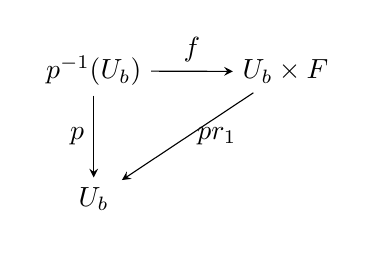
\begin{tikzpicture}
  \matrix (m) [matrix of math nodes,row sep=3em,column sep=3em,minimum width=2em]
  {
     {p^{-1}(U_b)} & {U_b \times F} \\
     U_b & \\};
  \path[-stealth]
    (m-1-1) edge node [above] {$f$}    (m-1-2)
            edge node [left]  {$p$}    (m-2-1)
    (m-1-2) edge node [right] {$pr_1$} (m-2-1);
\end{tikzpicture}
\end{center}
\end{definition}

\begin{definition} (Cartesian Product of Family over B).
Is a set $F$ of sections of the bundle with elimination map $app : F \times B \rightarrow E$ such that
\begin{equation}
F \times B \mapright{app} E \mapright{pr_1} B
\end{equation}
$pr_1$ is a product projection, so $pr_1$, $app$ are morphisms
of slice category $Set_{/B}$. The universal mapping property of $F$:
for all $A$ and morphism $A \times B \rightarrow E$ in $Set_{/B}$ exists
unique map $A \rightarrow F$ such that everything commute. So a category
with all dependent products is necessarily a category with all pullbacks.
\end{definition}

\begin{definition} (Trivial Fiber Bundle).
When total space $E$ is cartesian product $\Sigma(B,F)$ and $p = pr_1$
then such bundle is called trivial $(F,\Sigma(B,F),pr_1,B)$.
\end{definition}

\begin{theorem} (Functions Preserve Paths).
For a function $f: (x:A) \rightarrow B(x)$
there is an $ap_f : x =_A y \rightarrow f(x) =_{B(x)} f(y)$. This is called
application of $f$ to path or congruence property (for non-dependent case ---
$cong$ function). This property behaves functoriality
as if paths are groupoid morphisms and types are objects.
\end{theorem}

\begin{theorem} (Trivial Fiber equals Family of Sets).
Inverse image (fiber) of fiber bundle $(F,B*F,pr_1,B)$ in point $y:B$ equals $F(y)$.
\begin{lstlisting}
FiberPi (B: U) (F: B -> U) (y: B)
  : Path U (fiber (Sigma B F) B (pi1 B F) y)
           (F y)
\end{lstlisting}
\end{theorem}

\begin{theorem} (Homotopy Equivalence).
If fiber space is set for all base, and
there are two functions $f,g : (x:A) \rightarrow B(x)$ and two
homotopies between them, then these homotopies are equal.
\begin{lstlisting}
setPi (A: U) (B: A -> U)
    (h: (x: A) -> isSet (B x)) (f g: Pi A B)
    (p q: Path (Pi A B) f g)
  : Path (Path (Pi A B) f g) p q
\end{lstlisting}
\end{theorem}

Note that we will not be able to prove this theorem
until {\bf Issue III: Homotopy Type Theory} because
bi-invertible iso type will be announced there.

\subsubsection{$\Sigma$-type}

$\Sigma$ is a dependent sum type, the generalization of products.
$\Sigma$ type is a total space of fibration. Element of total
space is formed as a pair of basepoint and fibration.

\subsubsection*{Type-theoretical interpretation}

\begin{definition} ($\Sigma$-Formation).
\begin{lstlisting}
Sigma (A : U) (B : A -> U)
  : U = (x : A) * B x
\end{lstlisting}
\end{definition}

\begin{definition} ($\Sigma$-Introduction).
\begin{lstlisting}
dpair (A: U) (B: A -> U) (a: A) (b: B a)
  : Sigma A B = (a,b)
\end{lstlisting}
\end{definition}

\begin{definition} ($\Sigma$-Elimination).
\begin{lstlisting}
pr1 (A: U) (B: A -> U)
    (x: Sigma A B): A = x.1

pr2 (A: U) (B: A -> U)
    (x: Sigma A B): B (pr1 A B x) = x.2

sigInd (A: U) (B: A -> U)
       (C: Sigma A B -> U)
       (g: (a: A) (b: B a) -> C (a, b))
       (p: Sigma A B) : C p = g p.1 p.2
\end{lstlisting}
\end{definition}

\begin{theorem} ($\Sigma$-Computation).
\begin{lstlisting}
Beta1 (A: U) (B: A -> U)
      (a:A) (b: B a)
    : Equ A a (pr1 A B (a,b))

Beta2 (A: U) (B: A -> U)
      (a: A) (b: B a)
    : Equ (B a) b (pr2 A B (a,b))
\end{lstlisting}
\end{theorem}

\begin{theorem} ($\Sigma$-Uniqueness).
\begin{lstlisting}
Eta2 (A: U) (B: A -> U) (p: Sigma A B)
   : Equ (Sigma A B) p (pr1 A B p,pr2 A B p)
\end{lstlisting}
\end{theorem}

\subsubsection*{Categorical interpretation}

\begin{definition} (Dependent Sum).
The dependent sum along the morphism $f: A \rightarrow B$ in category $C$ is the left
adjoint $\Sigma_f : C_{/A} \rightarrow C_{/B}$ of the base change functor.
\end{definition}

\subsubsection*{Set-theoretical interpretation}

\begin{theorem} (Axiom of Choice).
If for all $x : A$ there is $y : B$ such that $R(x,y)$,
then there is a function $f : A \rightarrow B$
such that for all $x : A$ there is a witness of $R(x,f(x))$.
\begin{lstlisting}
ac (A B: U) (R: A -> B -> U)
 : (p: (x:A) -> (y:B)*(R x y))
-> (f:A->B) * ((x:A)->R(x)(f x))
\end{lstlisting}
\end{theorem}

\begin{theorem} (Total).
If fiber over base implies another fiber
over the same base then we can construct total space of section
over that base with another fiber.
\begin{lstlisting}
total (A:U) (B C: A -> U)
      (f: (x:A) -> B x -> C x) (w: Sigma A B)
    : Sigma A C = (w.1,f (w.1) (w.2))
\end{lstlisting}
\end{theorem}

\begin{theorem} ($\Sigma$-Contractability). If the fiber is set then the $\Sigma$ is set.
\begin{lstlisting}
setSig (A:U) (B: A -> U) (sA: isSet A)
       (sB : (x:A) -> isSet (B x))
     : isSet (Sigma A B)
\end{lstlisting}
\end{theorem}

\begin{theorem} (Path Between Sigmas).
Path between two sigmas $t,u: \Sigma(A,B)$ could be decomposed to
sigma of two paths $p:t_1=_{A}u_1)$ and $(t_2=_{B(p@i)}u_2)$.
\begin{lstlisting}
pathSig (A:U) (B : A -> U) (t u : Sigma A B)
      : Path U (Path (Sigma A B) t u)
               ((p: Path A t.1 u.1)
              * PathP (<i>B(p@i)) t.2 u.2)
\end{lstlisting}
\end{theorem}

\subsubsection{Path-type}

The Path identity type defines a Path space with elements and values.
Elements of that space are functions from interval $[0,1]$ to a values of that path space.
This ctt file reflects \footnote{Cyril Cohen, Thierry Coquand, Simon Huber, Anders M{\"{o}}rtberg. Cubical Type Theory: a constructive interpretation of the univalence axiom. 2015. \url{https://5ht.co/cubicaltt.pdf}}{CCHM} cubicaltt model with connections.
For \footnote{Carlo Angiuli, Brunerie, Coquand, Kuen-Bang Hou (Favonia), Robert Harper, Dan Licata. Cartesian Cubical Type Theory. 2017. \url{https://5ht.co/cctt.pdf}}{ABCFHL} yacctt model with
variables please refer to ytt file. You may also want to
read \footnote{Marc Bezem, Thierry Coquand, Simon Huber. A model of type theory in cubical sets. 2014. \url{http://www.cse.chalmers.se/~coquand/mod1.pdf}}{BCH},
\footnote{Carlo Angiuli, Kuen-Bang Hou (Favonia), Robert Harper. Cartesian Cubical Computational Type Theory: Constructive Reasoning with Paths and Equalities. 2018. \\ \url{https://www.cs.cmu.edu/~cangiuli/papers/ccctt.pdf}}{AFH}.
There is a \footnote{Andrew Pitts, Ian Orton. Axioms for Modelling Cubical Type Theory in a Topos. 2016. \url{https://arxiv.org/pdf/1712.04864.pdf}}{PO} paper about CCHM axiomatic in a topos.

\subsubsection*{Cubical interpretation}

Cubical interpretation was first given by Simon Huber\cite{Huber16} and later was
written first constructive type checker in the world by Anders M{\"{o}}rtberg\cite{Mortberg17}.

\begin{definition} (Path Formation).
\begin{lstlisting}
Hetero (A B: U)(a: A)(b: B)(P: Path U A B)
  : U = PathP P a b
Path (A: U) (a b: A)
  : U = PathP (<i> A) a b
\end{lstlisting}
\end{definition}

\begin{definition} (Path Reflexivity).
Returns an element of reflexivity path space for a given value of the type.
The inhabitant of that path space is the lambda on the homotopy
interval $[0,1]$ that returns a constant value a. Written in
syntax as |<i>a| which equals to $\lambda\ (i: I) \rightarrow a$.
\begin{lstlisting}
refl (A: U) (a: A) : Path A a a
\end{lstlisting}
\end{definition}

\begin{definition} (Path Application).
You can apply face to path.
\begin{lstlisting}
app1 (A: U)(a b:A)(p:Path A a b):A=p@0
app2 (A: U)(a b:A)(p:Path A a b):A=p@1
\end{lstlisting}
\end{definition}

\begin{definition} (Path Composition).
Composition operation allows to build a new path by given to paths
in a connected point.
\begin{center}
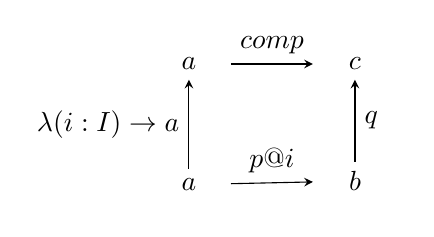
\begin{tikzpicture}
  \matrix (m) [matrix of math nodes,row sep=3em,column sep=3em,minimum width=3em]
  {
     a & c \\ % (1,1) (1,2)
     a & b \\ % (2,1) (2,2)
  };
  \path[-stealth]
    (m-1-1) edge node [above] {$comp$} (m-1-2)
    (m-2-1) edge node [left]  {$\lambda(i:I)\rightarrow a$} (m-1-1)
    (m-2-2) edge node [right] {$q$} (m-1-2)
    (m-2-1) edge node [above] {$p @ i$} (m-2-2);
\end{tikzpicture}
\end{center}
\begin{lstlisting}
composition
    (A: U) (a b c: A)
    (p: Path A a b) (q: Path A b c)
  : Path A a c
  = comp (<i>Path A a (q@i)) p []
\end{lstlisting}
\end{definition}

\begin{theorem} (Path Inversion).
\begin{lstlisting}
inv (A: U) (a b: A) (p: Path A a b)
  : Path A b a = <i> p @ -i
\end{lstlisting}
\end{theorem}

\begin{definition} (Connections).
Connections allows you to build square
with given only one element of path: i) $\lambda\ (i,j: I) \rightarrow p\ @\ min(i,j)$;
ii) $\lambda\ (i,j:I) \rightarrow p\ @\ max(i,j)$.
\begin{center}
  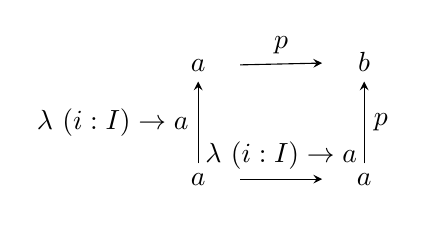
\begin{tikzpicture}
  \matrix (m) [matrix of math nodes,row sep=3em,column sep=3em,minimum width=3em]
  {
     a & b \\ % (1,1) (1,2)
     a & a                    \\ % (2,1) (2,2)
  };
  \path[-stealth]
    (m-1-1) edge node [above] {$p$}    (m-1-2)
    (m-2-1) edge node [left]  {$\lambda\ (i:I)\rightarrow a$}    (m-1-1)
    (m-2-2) edge node [right] {$p$} (m-1-2)
    (m-2-1) edge node [above] {$\lambda\ (i:I)\rightarrow a$} (m-2-2);
  \end{tikzpicture}
  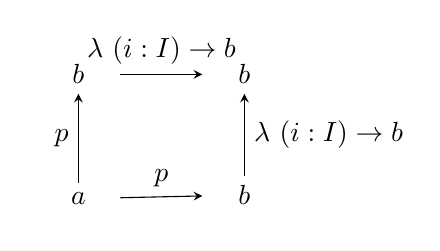
\begin{tikzpicture}
  \matrix (m) [matrix of math nodes,row sep=3em,column sep=3em,minimum width=3em]
  {
     b & b \\ % (1,1) (1,2)
     a & b                    \\ % (2,1) (2,2)
  };
  \path[-stealth]
    (m-1-1) edge node [above] {$\lambda\ (i:I) \rightarrow b$}    (m-1-2)
    (m-2-1) edge node [left]  {$p$}    (m-1-1)
    (m-2-2) edge node [right] {$\lambda\ (i:I) \rightarrow b$} (m-1-2)
    (m-2-1) edge node [above] {$p$} (m-2-2);
  \end{tikzpicture}
\end{center}
\begin{lstlisting}
meet (A: U) (a b: A) (p: Path A a b)
  : PathP (<x> Path A a (p@x)) (<i>a) p
  = <x y> p @ (x /\ y)

join (A: U) (a b: A) (p: Path A a b)
  : PathP (<x> Path A (p@x) b) p (<i>b)
  = <y x> p @ (x \/ y)
\end{lstlisting}
\end{definition}

\begin{theorem} (Congruence).
Is a map between values of one type
to path space of another type by an encode function between types.
Implemented as lambda defined on $[0,1]$ that returns
application of encode function to path application of
the given path to lamda argument |$\lambda$ (i:I) $\rightarrow$ f (p @ i)|
for both cases.
\begin{lstlisting}
ap  (A B: U) (f: A -> B)
    (a b: A) (p: Path A a b)
  : Path B (f a) (f b)

apd (A: U) (a x:A) (B: A -> U) (f: A -> B a)
    (b: B a) (p: Path A a x)
  : Path (B a) (f a) (f x)
\end{lstlisting}
\end{theorem}

\begin{theorem} (Transport).
Transports a value of the domain type to the value of the codomain type
by a given path element of the path space between domain and codomain types.
Defined as path composition with |[]| of a over a path $p$ --- |comp p a []|.
\begin{lstlisting}
trans (A B: U) (p: Path U A B) (a: A) : B
\end{lstlisting}
\end{theorem}

\subsubsection*{Type-theoretical interpretation}
\begin{definition} (Singleton).
\begin{lstlisting}
singl (A: U) (a: A): U = (x: A) * Path A a x
\end{lstlisting}
\end{definition}

\begin{theorem} (Singleton Instance).
\begin{lstlisting}
eta (A: U) (a: A): singl A a = (a,refl A a)
\end{lstlisting}
\end{theorem}

\begin{theorem} (Singleton Contractability).
\begin{lstlisting}
contr (A: U) (a b: A) (p: Path A a b)
  : Path (singl A a) (eta A a) (b,p)
  = <i> (p @ i,<j> p @ i/\j)
\end{lstlisting}
\end{theorem}

\begin{theorem} (Path Elimination, Diagonal).
\begin{lstlisting}
D (A: U) : U = (x y: A) -> Path A x y -> U
J (A: U) (x y: A) (C: D A)
  (d: C x x (refl A x))
  (p: Path A x y) : C x y p
= subst (singl A x) T (eta A x) (y, p)
        (contr A x y p) d where
  T (z: singl A x) : U = C x (z.1) (z.2)
\end{lstlisting}
\end{theorem}

\begin{theorem} (Path Elimination, Paulin-Mohring).
J is formulated in a form of Paulin-Mohring and implemented using
two facts that singleton are contractible and dependent function
transport.
\begin{lstlisting}
J (A: U) (a b: A)
  (P: singl A a -> U)
  (u: P (a,refl A a))
  (p: Path A a b) : P (b,p)
\end{lstlisting}
\end{theorem}

\begin{theorem} (Path Elimination, HoTT).
J from HoTT book.
\begin{lstlisting}
J (A: U) (a b: A)
  (C: (x: A) -> Path A a x -> U)
  (d: C a (refl A a))
  (p: Path A a b) : C b p
\end{lstlisting}
\end{theorem}

\begin{theorem} (Path Computation).
\begin{lstlisting}
trans_comp (A: U) (a: A)
  : Path A a (trans A A (<_> A) a)
  = fill (<i> A) a []
subst_comp (A: U) (P: A -> U) (a: A) (e: P a)
  : Path (P a) e (subst A P a a (refl A a) e)
  = trans_comp (P a) e
J_comp (A: U) (a: A) (C: (x: A)
 -> Path A a x -> U) (d: C a (refl A a))
  : Path (C a(refl A a)) d
         (J A a C d a(refl A a))
  = subst_comp (singl A a) T (eta A a) d
    where T (z:singl A a)
        : U = C a (z.1) (z.2)
\end{lstlisting}
\end{theorem}

Note that  Path type has no Eta rule due to groupoid interpretation.

\subsubsection*{Groupoid interpretation}

The groupoid interpretation of type theory is well known article by Martin Hofmann and Thomas Streicher,
more specific interpretation of identity type as infinity groupoid.
The groupoid interpretation of Path equality will be given along with category theory library
in {\bf Issue VII: Category Theory}.

\subsection{Universes}

This introduction is a bit wild strives to be simple yet precise.
As we defined a language BNF we could define a language AST by
using inductive types which is yet to be defined
in {\bf Issue II: Inductive Types and Models}. This SAR notation is due Barendregt.

\begin{definition} (Terms). Point in initial object of language AST
inductive definition is called a term. If type theory or language is defined as
an inductive type (AST) then the term is defined as its instance.
\end{definition}

\begin{definition} (Sorts). N-indexed set of universes $\mathrm{U}_{n \in \mathrm{N}}$.
Could have any number of elements which defines different type systems. All built-in
types as long as user defined types are landed usually by default in $U_0$ universe.
Sorts represented in type checker as a separate constructor.
\end{definition}

\begin{definition} (Axioms). The inclusion rules {\bf $\mathrm{U_i : U_j}, i,j \in \mathrm{N}$},
that define which universe is element of another given universe. You may attach
any rules that joins $i,j$ in some way. Axioms with sorts define universe hierarchy.
\end{definition}

\begin{definition} (Rules). The set of landings
$\mathrm{U_i} \rightarrow \mathrm{U_j} : \mathrm{U_{\lambda(i,j), i,j \in \mathrm{N}}}$,
where $\mathrm{\lambda : N \times N \rightarrow N}$. These rules define term dependence or
how we land (in which universe) formation rules in definitions.
\end{definition}

\begin{definition} (Predicative hierarchy). If $\mathrm{\lambda}$ in Rules
is an uncurried function $\mathrm{max : N \times N \rightarrow N}$
then such universe hierarchy is called predicative.
\end{definition}

\begin{definition} (Impredicative hierarchy). If $\lambda$ in Rules
is a second projection of a tuple $\mathrm{snd : N \times N \rightarrow N}$
then such universe hierarchy is called impredicative.
\end{definition}

\begin{definition} (Definitional Equality). For any $\mathrm{U}_i, i \in \mathrm{N}$ there is
defined an equality between its members and between its instances.
For all x,y $\in$ A, there is defined a x=y. Definitional equality
compares normalized term instances.
\end{definition}

\begin{definition} (SAR). The universum space is configured with a triple of:
i) sorts, a set of universes  $\mathrm{U}_{n \in \mathrm{N}}$ indexed over set N;
ii) axioms, a set of inclusions {\bf $\mathrm{U_i : U_j}, i,j \in \mathrm{N}$};
iii) rules of term dependence universe landing, a set of landings
$\mathrm{U_i} \rightarrow \mathrm{U_j} : \mathrm{U_{\lambda(i,j), i,j \in \mathrm{N}}}$, where $\lambda$ could be function $max$ (predicative) or $snd$ (impredicative).
\end{definition}

\begin{example} (CoC). SAR = $\{ \{\star , \Box \},\{ \star : \Box \},
        \{ i \rightarrow j : j; i, j \in \{ \star, \Box \}
        \}$. Terms live in universe $\star$, and types live in universe $\Box$. In CoC $\mathrm{\lambda=snd}$.
\end{example}

\begin{example} ($\mathrm{PTS}^\infty$, $\mathrm{MLTT}^\infty$).\\ SAR = $\{ \mathrm{U}_{i \in \mathrm{N}},
    \mathrm{U_i : U_{j; i < j; i,j \in N}},
    \mathrm{U_i} \rightarrow \mathrm{U_j} : \mathrm{U_{\lambda(i,j); i,j \in \mathrm{N}}}
    \}$. Where $U_i$ is a universe of $i$-level or $i$-category in categorical interpretation.
    The working prototype of $\mathrm{PTS}^\infty$ is given in
    {\bf Addendum I: Pure Type System for Erlang}\cite{Tonpa18}.
\end{example}

\subsection{Contexts}

Speaking of type checker execution, we introduce context or dictionary with types and terms,
from which we can derive typed variables. This chain could be implemented as
nested sigma types (due to R.A.G.Seely) or list types (due to Voevodsky). Categorically
dependent type theory is built upon categories of contexts.

\begin{definition} (Empty Context).
$$
    \gamma_0 : \Gamma =_{def} \star.
$$
\end{definition}

\begin{definition} (Context Comprehension).
$$
\Gamma\ ; A =_{def} \sum_{\gamma:\Gamma}A(\gamma).
$$
\end{definition}

\begin{definition} (Context Derivability).
$$
\Gamma \vdash A =_{def} \prod_{\gamma:\Gamma}A(\gamma).
$$
\end{definition}

\subsection{MLTT}

Here is given formal model of type-theoretical interpretation of Martin-Löf Type Theory.
It combines 4 Path rules (no eta), 5 $\Pi$ rules, and 6 $\Sigma$ rules (two elims).
The proof is provided by direct embedding (internalizing) the model intro the model
of type checker which is even more powerful.

\begin{definition} (MLTT).
The MLTT as a Type is defined by taking all rules
for $\Pi$, $\Sigma$ and Path types into one $\Sigma$ telescope or context.
\begin{lstlisting}[mathescape=true]
MLTT (A: U): U
  = (Pi_Former: (A -> U) -> U)
  * (Pi_Intro: (B: A -> U) (a: A)
    -> B a -> (A -> B a))
  * (Pi_Elim: (B: A -> U) (a: A)
    -> (A -> B a) -> B a)
  * (Pi_Comp1: (B: A -> U) (a: A)
    (f: A -> B a) -> Path (B a)
    (Pi_Elim B a(Pi_Intro B a(f a)))(f a))
  * (Pi_Comp2: (B: A -> U) (a: A)
    (f: A -> B a) ->
    Path (A -> B a) f (\(x:A) -> f x))
  * (Sigma_Former: (A -> U) -> U)
  * (Sigma_Intro: (B: A -> U) (a: A)
    -> (b: B a) -> Sigma A B)
  * (Sigma_Elim1: (B: A -> U)
    (_: Sigma A B) -> A)
  * (Sigma_Elim2: (B: A -> U)
    (x: Sigma A B) -> B (pr1 A B x))
  * (Sigma_Comp1: (B: A -> U) (a: A)
    (b: B a) -> Path A a (Sigma_Elim1 B
                  (Sigma_Intro B a b)))
  * (Sigma_Comp2: (B: A -> U) (a: A)
    (b: B a) -> Path (B a) b
    (Sigma_Elim2 B (a,b)))
  * (Sigma_Comp3: (B: A -> U) (p: Sigma A B)
    -> Path (Sigma A B) p
            (pr1 A B p,pr2 A B p))
  * (Id_Former: A -> A -> U)
  * (Id_Intro: (a: A) -> Path A a a)
  * (Id_Elim: (x: A) (C: D A)
    (d: C x x (Id_Intro x))
    (y: A) (p: Path A x y) -> C x y p)
  * (Id_Comp: (a:A)(C: D A)
    (d: C a a (Id_Intro a)) ->
    Path (C a a (Id_Intro a)) d
         (Id_Elim a C d a (Id_Intro a)))
  * U
\end{lstlisting}
\end{definition}

\begin{theorem} (Model Check).
There is an instance of MLTT.
\begin{lstlisting}
instance (A: U): MLTT A
  = (Pi A,    lam A, app A,
              Beta A, Eta A,
     Sigma A, dpair A, pr1 A, pr2 A,
              Beta1 A, Beta2 A, Eta2 A,
     Path A,  refl A, J A,
              J_comp A, A)
\end{lstlisting}
\end{theorem}

\subsection*{Cubical Model Check}

The result of the work is a |mltt.ctt| file which can be runned using |cubicaltt|.
Note that computation rules take a seconds to type check.

\begin{lstlisting}
cubicaltt -- 6 second.
Arend -- 1 second.
Agda (cubical) -- & 2 second.
\end{lstlisting}

\subsection*{Conclusions}

In this issue the type-theoretical model (interpretation) of MLTT was
presented in cubical syntax and type checked in it.
This is the first constructive proof of internalization of MLTT.

From the theoretical point of view the landspace of possible interpretation was shown
corresponding different mathematical theories for those who are new to type theory.
The brief description of the previous attempts to internalize MLTT could
be found as canonical example in MLTT works, but none of them give the constructive
J eliminator or its equality rule. As a selected prover for the article wa
chosen cubicaltt but this excersise was implemented on all current
cubical type checkers\footnote{https://cubical.systems}:
Arend\footnote{https://github.com/groupoid/arend},
Agda\footnote{https://github.com/groupoid/agda},
cubicaltt\footnote{https://github.com/groupoid/cubical},
yacctt, redtt, RedPRL, Lean\footnote{https://github.com/groupoid/lean}.
Type theoretical cubical constructions was given for the Path types
along the article for other interpretations, all of them were taken from our Groupoing
Infinity\footnote{https://groupoid.space/mltt/types/} base library.

\begin{table}[!ht]
  \centering
  \caption*{\textbf{Table}. Core Features}
  \begin{adjustbox}{width=\columnwidth,center}
  \begin{tabular}{lccccccc}
    \hline
       Lang          & Pi & Sigma & Eq & Path & U^{\infty} & Co/Fix & Lazy\\
    \hline
       PTS           & x\\
       Cedile, MLTT  & x & x & x\\
       PTS^{\infty}  & x &   &   &   & x\\
       \textbf{MLTT^{$\infty$}} & x & x &   & x & x\\
       \textbf{Lean, Agda}    & x &   & x & x & x\\
       NuPRL         & x & x & x &   &   & x\\
       System-D      & x & x &   &   &   & x & x\\
       \textbf{cubical}       & x & x & x & x &   & x\\
  \end{tabular}
  \end{adjustbox}
\end{table}

The objective of complete derivability of all eliminators, computational and uniquness rules
is a basic objective for constructive mathematics as mathematical reasoning implies verification
and mechanization. Yes cubical type system represent most compact system that make possible
derivability of all theorems for core types which make this system as a first candidate for
the metacircular type checker.

Also for programming purposes we may also want to investigate Fixpoint as a useful
type in coinductive and modal type theories and harmful type in theoretical foundation of type systems.
Elimination the possibility of uncontrolled Fixpoint is a main objective of the correct type system
for reasoning without paradoxes. By this creatiria we could filter all the fixpoint implementations being condidered harmful.

Without a doubt the core type that makes type theory more
like programming is the inductive type system that allows to
define type families. In the following Issue II will be shown
the semantics and embedding of inductive types with several types
of Inductive-Recursive encodings.

\begin{table}[!ht]
  \centering
  \caption*{\textbf{Table}. Inductive Type Systems}
  \begin{adjustbox}{width=\columnwidth,center}
  \begin{tabular}{lccc}
    \hline
       Lang & Co/Inductive & Quot/Trunc & HITs\\
    \hline
       System-D & x\\
       Lean & x & x\\
       NuPRL & x & x\\
       Arend & x & x & x\\
       Agda, Coq & x & & x\\
       cubicaltt, yacctt, RedPRL & x & & x\\
  \end{tabular}
  \end{adjustbox}
\end{table}

Further research of the most pure type theory on a weak fibrations and pure Kan
oprations without interval lattice structure (connections, de Morgan algebra, connection
algebras) and diagonal coersions could be made on the way of building a minimal homotopy core\cite{Cavallo19}.

\begin{table}[!ht]
  \centering
  \caption*{\textbf{Table}. Cubical Type Systems}
  \begin{adjustbox}{width=\columnwidth,center}
  \begin{tabular}{lccc}
    \hline
       Lang & Interval & Diagonal & Kan/Coe\\
    \hline
       BCH, cubical        & & & $0\rightarrow r$, $1 \rightarrow r$\\
       CCHM, cubicaltt, Agda       & $\lor$,$\land$ & & $0 \rightarrow 1$\\
       Dedekind          & $\lor$,$\land$ & & $0 \rightarrow 1$, $1 \rightarrow 0$\\
       AFH/ABCFHL, yacctt & & x & $r \rightarrow s$\\
       HTS/CMS    & &   & $r \rightarrow s$, $weak$\\
  \end{tabular}
  \end{adjustbox}
\end{table}

The next language after PTS$^{\infty}$ and MLTT$^{\infty}$ will
be HTS$^{\infty}$ with recursive higher inductive type system and infinite number of universes.
Along with O-CPS interpreter this evaluators form a set of languages as a part of conceptual model of theorem
proving system with formalized virtual machine as extraction target.

\subsection*{Further Research}

This article opens the door to a series that will unvail the different topics of
homotopy type theory with practical emphasis to cubical type checkers.
The Foundations volume of articles define formal programming language
with geometric foundations and show how to prove properties of such constructions.
The second volume of article is dedicated to cover the programming and modeling of Mathematics.

\subsubsection*{\hspace{0.5cm}Foundations I--V, Mathematics VI--X}

\hspace{0.4cm} {\bf Issue I: Intenalizing Martin-Löf Type Theory}.
The first volume of definitions gathered into one article dedicated to
various $\prod$ and $\sum$ properties and internalization of MLTT in the host language typechecker.

{\bf Issue II: Inductive Types and Encodings}.
This episode tales a story of inductive types, their encodings,
induction principle and its models.

{\bf Issue III: Homotopy Type Theory}.
This issue is try to present the Homotopy Type Theory without higher inductive types
to neglect the core and principles of homotopical proofs.

{\bf Issue IV: Higher Inductive Types}.
The metamodel of HIT is a theory of CW-complexes. The category of HIT is a homotopy category.
This volume finalizes the building of the computational theory.

{\bf Issue V: Modalities}. The constructive extensions with additional context and
adjoint transports between toposes (cohesive toposes). This approach serves the needs
of modal logics, differential geometry, cohomology.

%The main intention of Foundation volume is to show the internal language
%of working topos of CW-complexes, the construction of fibrational sheaf type theory.

%\subsubsection*{Mathematics}

%The second volume of article is dedicated to cover the mathematical
%programming and modeling.

\indent {\bf Issue VI: Set Theory}.
The set theory and mere propositions: set, prop.

{\bf Issue VII: Category Theory}.
The model of Category Theory definitions.

{\bf Issue VIII: Topos Theory}.
Formal packaging of set theory in a topos. Formal Topos and Formal Sheaf.
It also includes sheaf embedding of type theory in type theory.

{\bf Issue IX: Algebraic Topology}. This branch of study of topological spaces with abstract algebra
includes followin areas: Homotopy Theory, Homological Algebra, Complexes,

{\bf Issue X: Differential Geometry}. This branch of study includes
infinitesimal constructions and Cartan geometry, the chapter is
slightly base on Felix Wellen dissertation.

\twocolumn[

  \begin{@twocolumnfalse}


   \renewcommand{\bibname}{\fontsize{10pt}{12pt}\selectfont References}
   \bibliographystyle{ieeetr}
   \def\bibfont{\fontsize{8}{10}\selectfont}
    \bibliography{mltt}
   \vspace{1cm}

  \setmainfont{Arial}
  \parindent=2em

  \fontsize{8pt}{10pt}\selectfont \textrf{М.Е.Сохацький}\\
  \vspace{0.1cm}
  \fontsize{9pt}{11pt}\selectfont \indent ВИПУСК 1: ВБУДОВУВАННЯ ТЕОРІЇ ТИПІВ МАРТІНА-ЛЬОФА

{\bf Проблематика.}
Був пройдений довгий шлях від чистих типових систем AUTOMATH де Брейна до
гомотопічних типових верифікаторів. Ця стаття стосується тільки формального ядра
теорії типів Мартіна-Льофа: $\Pi$ и $\Sigma$ типів (які відповідають
квантору загальності $\forall$ та квантору існування $\exists$ у класичній логіці)
та типу-рівності.\\
\indent {\bf Мета дослідження.}
Визначити типову систему як частину концептуальної моделі системи доведення теорем,
у якій конструктивно виражається J елімінатор та його теореми, спираючись на більш абстрактні
примітиви типа рівності. Це стало можливим завдяки кубічній теорії типів (2016) та типовому кубічному верифікатору
{\bf cubicaltt}\footnote{http://github.com/mortberg/cubicaltt} (2017).
Ціль статті --- продемонструвати формальне вбудовування теорії типів Мартіна-Льофа
в виконуючу авторську кубічну типову систему MLTT$^{\infty}$ з повним набором правил виводу.\\
\indent {\bf Методика реалізації.}
Так як всі типи в теорії формулюються за допомогою п'яти
правил: формації, інтро, елімінації, обчисленя, рівності) що в сутності
є кодуванням ізоморфізмами ініальних об'єктів в категорія F-алгебр, ми зконструювали
номінальні типи-синоніми для виконуючого верифікатора та довели, що це є реалізацією MLTT.
Так як не всі можуть бути знайомі з теорією типів,
це випуск також містить їх інтерпретації з точки зору різних розділів математики.\\
\indent {\bf Результати дослідження.}
Ця робота веде до декількох результатів:
1) MLTT$^{\infty}$ --- спеціальна версія теорії типів Мартіна-Льофа зі зліченною кількістю всесвітів та Path типом без eta-правила для HoTT застосування у яку ми будем вбудовувати класичну MLTT;
2) Власе сама інтерналізація MLTT в MLTT$^{\infty}$ з синтаксисом який дозволяє виводити поліморфні всесвіти;
3) Класифіковані різні інтерпретації цієї системи типів: теоретико-типова, категорна або топосо-теоретична, гомотопічна або кубічна;
4) Як результат цей випуск відкриває серію статей по формалізації різних розділів математики,
   та присвячений формалізації основам математики в кубічній теорії типів, MLTT моделюванню та кубічній верифікації;
5) Це може розглядатися як універсальний тест для імплементації типового верифікатора,
позаяк компенсаця інтро правила та правила елімінатора пов'язані в правилі
обчислення та рівності (бета та ета редукціях). Таким чином, доводжучи реалізацію MLTT,
ми доводимо властивості самого виконуючого верифікатора;
6) Завдяки позитивним результатм кубічна теорія була вибрана як геометричне розширення системи індуктивних типів
для математичної верифікації як частина концептуальної системи доведення теорем, яка включатимиме серію мов
як середовище верифікації.\\

  \end{@twocolumnfalse}

]

\twocolumn[

  \begin{@twocolumnfalse}

  \parindent=2em
  \setmainfont{Arial}
  \fontsize{9pt}{11pt}\selectfont

\indent {\bf Висновки.}
Додамо, що це тільки вхід в техніку прямого вбудовування і після MLTT моделювання,
ми можем піднятися вище — до вбудовування в систему індуктивних типів, і далі,
до вбудовування CW-комплексів як зклейок вищих індуктивних типів, та далі до модальних логік.
Це означає широкий спектр математичних теорії всередині HoTT аж до алегбраїчної топології.
Подальша рефлексія веде до комбінації різних типових підсистем в спектральних категорія мовних рівнів
з модулями-плагінами для синтаксичних розширень та алгоритмів нормалізації програм в цих синтаксисах. \\
\indent {\bf Ключові слова:} Теорія типів Мартіна-Льофа, Кубічна теорія типів.
\vspace{1cm}


 \setmainfont{Arial}
\fontsize{8pt}{10pt}\selectfont \textrf{М.Э.Сохацкий}\\
    \vspace{0.1cm}
\fontsize{9pt}{11pt}\selectfont \hspace{0.53cm} ВЫПУСК 1: ВСТРАИВАНИЕ ТЕОРИИ ТИПОВ МАРТИНА-ЛЁФА

 \setmainfont{Arial}


{\bf Проблематика.}
Был пройден долгих путь от чистых типовых систем AUTOMATH де Брейна до
гомотопических типовых верификаторов. Эта статья затрагивает только формализацию
ядра теории типов Мартина-Лёфа: $\Pi$ и $\Sigma$ типов (которые соотвествуют
квантору всеобщности $\forall$ и квантору существования $\exists$ в классической логике)
и типу-равенству.\\
\indent {\bf Цель исследования.}
Определить типовую систему для концептуальной модели системы доказательства теорем,
в которой конструктивно выражетается J элиминатор и его теоремы, опираясь на более абстрактные
примитивы типа равенства. Это стало возможным благодаря кубической интерпретации и двум
статьям по кубической теории типов и по кубическому верификатору. Также стояла задача
исследовать различные кубические системы типов для выбора своей минимальной подсистемы способной встроить MLTT.
Цель статьи -- демонстрация формального встраивания теории типов Мартина-Лёфа в авторскую кубическую
систему MLTT$^{\infty}$ с полным набором правил вывода.\\
\indent {\bf Методика реализации.}
Так как все типы в теории формулируются с помощью пяти
правил: формации, интро, элиминации, вычисления, уникальности), что по существу
есть кодированием изоморфизмами инициальных объектов в категориях F-алгебр, мы построили
номиналные типы-синонимы для исполняющего верификатора и доказали, что это является реализацией MLTT.
Так как не все могут быть знакомы с теорией типов, этот выпуск также включает интерпретации с точки
зрения различных разделов математики.\\
\indent {\bf Результаты исследования.}
Эта робота ведет к нескольким результатам:
1) MLTT$^{\infty}$ --- специальная версия теории типов Мартина-Лёфа со счетным количеством вселенных
   и Path типом без eta-правила для HoTT применений, в которую будет произведено встраивание классической MLTT;
2) Собственно сама интернализация MLTT в MLTT$^{\infty}$ с полиморфными вселенными;
3) Классификованы разные интерпретации этой системы типов: теоретико-типовая, категорная або топосо-теоретическая, гомотопическая или кубическая;
4) Как результат этот выпуск открывает серию статей по формализации разных разделов математики,
   которые посвящены формализации основам математики в кубической теории типов, MLTT моделюванию и кубической верификации;
5) Это может также рассмартриваться как универсальний тест для имплементации типового верификатора,
как как компенсация интро правила и правила элиминации связаны в правилах бета и эта редукции, таким образом
мы доказываем правила самого верификатора;
6) Благодаря позитивным результатам, кубическая теория была выбрана как геометрическое расширение системы индуктивных
типов для маметамтической механизируемой верификации как часть более общей работы --- концептуальной системы
доказательства теорем, которая включает в себя серию языков и языковых средств как среду для верификации и экстракции доказанных программ.\\
\indent {\bf Выводы.}
Заметим, что это только вход в технику прямого встраивания и после MLTT моделирования мы можем
поднятся выше — до встраивания в систему индуктивных типов, и далее, до встраивание CW-комплексов как
склее высших индуктивных типов, и далее до модальных логик.
Это означает широкий спектр математических теорий внутри самой HoTT вплоть до алгебраической топологии и дифференциальной геометрии.
Дальнейшая рефлекция ведет к рассмотрению комбинаций типовых подсистем в спектральных категория языковых уравней
с модулями-плагинами для синтаксических расширений и алгоримов нормализации программ в этих синтаксисах. \\
\indent {\bf Ключевые слова:} Теория типов Мартина-Лёфа, Кубическая теория типов.

 \end{@twocolumnfalse}

]

\end{document}

